\documentclass[aspectratio=169,11pt]{beamer}
\usepackage[T1]{fontenc}
\usepackage[utf8]{inputenc}
\usepackage{lmodern,amsmath,amssymb,graphicx,tikz}
\usetikzlibrary{arrows.meta,calc}
\usetheme{default}
\usefonttheme{serif}
\setbeamercolor{normal text}{fg=black,bg=white}
\setbeamercolor{structure}{fg=black}
\setbeamercolor{frametitle}{fg=black}
\setbeamercolor{title}{fg=black}
\setbeamertemplate{navigation symbols}{}
\setbeamertemplate{footline}[frame number]
\setbeamertemplate{itemize items}[circle]
\setbeamersize{text margin left=8mm,text margin right=8mm}
\setlength{\parskip}{5pt}
\newcommand{\cO}{\mathcal O}
\newcommand{\cI}{\mathcal I}
\newcommand{\cA}{\mathcal A}
\newcommand{\db}{\bar\partial}
\newcommand{\C}{\mathbb C}
\newcommand{\Pj}{\mathbb P}
\newcommand{\norm}[1]{\lVert#1\rVert}
\newcommand{\src}[1]{\par\vfill{\scriptsize #1\par}}
\author{Daniel Gonz\'alez Casanova Azuela}

\title{Kodaira embedding theorem (Part 2)}
\subtitle{From solving \(\bar\partial\) to homogeneous polynomial equations}
\date{Hodge theory, IMPA \quad 16 November 2026}
\begin{document}

\begin{frame}\titlepage\end{frame}

\begin{frame}{Today: Kodaira embedding}
Let \(L\) be a positive holomorphic line bundle on a compact complex manifold \(X\).
For all sufficiently large \(N\), the complete linear system gives an embedding
\[
\boxed{\Phi_N:X\hookrightarrow\Pj(H^0(X,L^N)^*).}
\]
\par\bigskip
\textbf{What remains:} construct singular metrics with the prescribed ideals and positive curvature.
\src{Demailly, CIME notes, Exercise 5.14 and Theorem 5.15.}
\end{frame}

\begin{frame}{Kunihiko Kodaira}
\begin{columns}[c]
\column{.42\textwidth}
\centering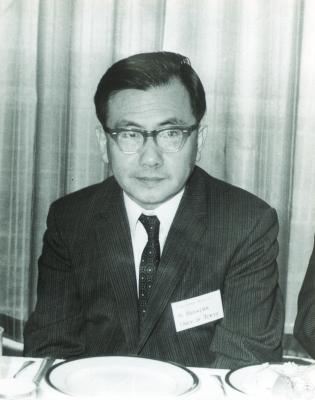
\includegraphics[height=4.7cm]{../assets/Kunihiko_Kodaira.png}
\column{.54\textwidth}
\textbf{Analysis supplies projective coordinates.}
\par\bigskip
The embedding theorem turns positivity of a Hermitian metric into a global algebraic description.
\par\bigskip
Kodaira received the Fields Medal in 1954.
\end{columns}
\src{Photo: Konrad Jacobs / MFO, Tokyo 1969, CC BY-SA 2.0 DE. Historical source: IAS scholar profile.}
\end{frame}

\begin{frame}{Lecture 23 (Daniel): what we wanted}
\textbf{The geometric goal.} Use global sections of a positive line bundle to embed \(X\) into projective space.
\par\bigskip
\textbf{The reduction.} We need sections with prescribed values and first derivatives.
\par\bigskip
The long exact sequence reduced those prescriptions to
\[
H^1(X,A\otimes I)=0.
\]
Here \(A\) is the bundle whose sections we want, and \(I\) records the vanishing conditions.
\par\medskip
We also recalled smooth Kodaira vanishing, using harmonic representatives and \(\omega=i\Theta_B\).
\end{frame}

\begin{frame}{Our priority today}
\begin{enumerate}
\setlength{\itemsep}{14pt}
\item Finish the local example: which functions survive the singular norm?
\item Explain how an estimate produces a solution of \(\db u=f\).
\item Use that solution to build separating sections and an embedding.
\item Use Chow to turn the analytic image into homogeneous polynomial equations.
\end{enumerate}
\par\medskip
Kawamata--Viehweg is an optional continuation after this argument is clear.
\end{frame}

\begin{frame}{The example: recover the meaning of the letters}
We are near \(x=0\) in \(\C^n\). Choose the metric with weight \(\varphi=a\log|z|\).
\[
|f|_h^2=\frac{|f|^2}{|z|^{2a}},\qquad
\boxed{f\in\cI(h)_0\iff k>a-n.}
\]
\begin{itemize}
\setlength{\itemsep}{10pt}
\item \(n\) is the complex dimension.
\item \(a\) is the coefficient we choose in the metric.
\item \(k=\operatorname{ord}_0(f)\) is the first nonzero Taylor degree, so \(k\) is a nonnegative integer (for \(f\ne0\)).
\end{itemize}
We use the criterion from lecture 23 (Daniel), without redoing its integral.
\end{frame}

\begin{frame}{Choose the coefficient: first the maximal ideal}
Choose \(a=n\). Substitute into the criterion:
\[
k>a-n=n-n=0.
\]
Since \(k\) is an integer, this says \(k\ge1\), equivalently \(f(0)=0\).
\[
\boxed{a=n\quad\Longrightarrow\quad\cI(h)_0=\mathfrak m_0.}
\]
Constants are excluded. Linear, quadratic, and higher-order terms are allowed.
\par\medskip
This means vanishing to order \textbf{at least one}, not necessarily exactly one.
\end{frame}

\begin{frame}{Choose the coefficient: now the square}
Choose \(a=n+1\). Substitute again:
\[
k>a-n=(n+1)-n=1.
\]
Now \(k\ge2\): both the constant and linear Taylor terms vanish.
\[
\boxed{a=n+1\quad\Longrightarrow\quad\cI(h)_0=\mathfrak m_0^2.}
\]
\textbf{In \(\C^2\):} at \(a=2\), constants fail but linear terms survive. At \(a=3\), linear terms fail too.
\par\medskip
Equality in the integrability threshold is excluded.
\end{frame}



\begin{frame}{First jets: why quotient by the square?}
In coordinates centred at \(x\), a holomorphic function has Taylor expansion
\[
f(z)=f(0)+\sum_{j=1}^n\frac{\partial f}{\partial z_j}(0)z_j
       +\text{terms of degree at least }2.
\]
The terms of degree at least \(2\) belong to \(\mathfrak m_x^2\).
\par\medskip
So reduction modulo \(\mathfrak m_x^2\) remembers exactly the value and first derivatives. This is the \textbf{first jet}.
\par\medskip
Surjectivity onto this quotient lets us prescribe these data independently.
\end{frame}

\begin{frame}{First jets: what the quotient remembers}
In \(\C^2\), for example,
\[
f(z_1,z_2)=c+b_1z_1+b_2z_2+\text{terms in }\mathfrak m_0^2.
\]
So
\[
\cO_{X,0}/\mathfrak m_0^2\simeq\C\oplus T_0^*X
\]
via value and differential. We can prescribe \(c\), \(b_1\), \(b_2\) independently.
\par\medskip
The \textbf{ideal} is the error we may add without changing the first jet. The \textbf{quotient} is the first-jet data themselves.
\end{frame}

\begin{frame}{The theorem we can now use: Nadel}
Let \((X,\omega)\) be compact Kähler. Let \(B\) have a singular metric \(h\) with
\[
i\Theta_h\ge\varepsilon\omega,\qquad\varepsilon>0.
\]
Then
\[
\boxed{H^q(X,K_X\otimes B\otimes\cI(h))=0\quad(q>0).}
\]
\textbf{What we saw in lecture 23 (Daniel).} Weighted forms compute this cohomology. Weighted \(L^2\) solvability makes closed forms exact.
\par\smallskip
The singular-weight solvability and local lemma remain analytic inputs.
\src{Demailly, CIME notes, Corollary 5.3 and Theorem 5.11.}
\end{frame}

\begin{frame}{Alan Michael Nadel}
\begin{columns}[c]
\column{.44\textwidth}
\centering

\begin{tikzpicture}
\fill[black!12] (.12,-.12) rectangle (4.32,5.08);
\filldraw[fill=blue!4,draw=blue!50!black] (0,0) rectangle (4.2,5.2);
\draw[blue!50!black,line width=2pt] (.2,0)--(.2,5.2);
\node[align=center,text width=3.6cm] at (2.2,4.65) {\small\textsc{Annals of Mathematics}};
\draw[blue!40] (.6,4.15)--(3.8,4.15);
\node[align=center,text width=3.3cm] at (2.2,3.0) {\small\emph{Multiplier ideal sheaves and Kähler--Einstein metrics of positive scalar curvature}};
\node[align=center] at (2.2,1.5) {\small Alan Michael Nadel};
\node at (2.2,.6) {\Large\textbf{1990}};
\end{tikzpicture}
\column{.52\textwidth}
\begin{itemize}
\setlength{\itemsep}{16pt}
\item His 1990 paper introduced multiplier ideal sheaves while studying \textbf{Kähler--Einstein metrics}.
\item He was a student of \textbf{Yum-Tong Siu} at Harvard: PhD in 1988, with the thesis \emph{Hyperbolic Surfaces}.
\item His paper connects the failure of analytic estimates with an ideal sheaf, inspired by Kohn's multipliers.
\end{itemize}
\end{columns}
\src{Nadel, Ann. of Math. 132 (1990), 549--596, abstract. Mathematics Genealogy Project, id 175682. Searches of 13 Nov 2026: Oberwolfach Photo Collection, Wikimedia Commons, Wikipedia. Illustration based on the bibliographic record.}
\end{frame}

\begin{frame}{Why the kernel contains the canonical bundle}
Let \(e\) be a local holomorphic frame of \(B\), with \(|e|_h^2=e^{-2\varphi}\).
A \(B\)-valued \((n,0)\)-form is locally
\[
u=f\,dz_1\wedge\cdots\wedge dz_n\otimes e.
\]
The factor \(dz_1\wedge\cdots\wedge dz_n\) is a local frame of \(K_X\).
\par\medskip
Thus \(u\) is a section of \(K_X\otimes B\). Since both frames are holomorphic,
\[
\db u=0\quad\Longleftrightarrow\quad\db f=0.
\]
\end{frame}

\begin{frame}{A short reminder: weak derivatives}
A locally integrable function need not have classical derivatives. Its derivative is defined by testing against smooth compactly supported functions:
\[
\langle\partial_jf,\eta\rangle=-\int f\,\partial_j\eta.
\]
This is integration by parts, used as a definition.
\par\medskip
\(\db f=0\) \textbf{weakly} means the corresponding tested identities vanish.
A standard local regularity fact for the Cauchy--Riemann equations says that such an \(f\) is holomorphic, up to equality almost everywhere.
\par\medskip
The singular metric changes which forms have finite norm. Weak derivatives let us work with nonsmooth forms.
\end{frame}

\begin{frame}{Why the kernel contains exactly the multiplier ideal}
For the form \(u=f\,dz_1\wedge\cdots\wedge dz_n\otimes e\), local square integrability means
\[
\int|f|^2e^{-2\varphi}\,d\lambda<\infty,
\]
up to a smooth positive factor from the coordinates and background metric.
\par\medskip
If \(\db u=0\), then \(f\) is holomorphic. The displayed condition is precisely \(f\in\cI(h)\).
\[
\boxed{\ker(\db:\mathcal L^{n,0}\to\mathcal L^{n,1})
=K_X\otimes B\otimes\cI(h).}
\]
Here \(\mathcal L^{n,q}\) consists of forms \(u\) for which \(u\) and \(\db u\) are locally \(L^2\). Both directions follow from the local expression.
\src{Demailly, CIME notes, proof of Theorem 5.11.}
\end{frame}

\begin{frame}{Local exactness and global solvability are different}
\textbf{Locally:} the weighted Poincaré lemma makes the complex of \(L^2\) forms a resolution of \(K_X\otimes B\otimes\cI(h)\).
\par\medskip
Smooth cutoffs preserve its sheaves: \(\db(\chi u)=\db\chi\wedge u+\chi\db u\). Thus they are fine, and the resolution computes sheaf cohomology.
\par\medskip
\textbf{Globally:} we must solve \(\db u=f\) for every closed \(f\) of positive degree.
\par\medskip
The curvature estimate and the Hilbert-space argument provide that global solution.
\end{frame}

\begin{frame}{The Hilbert-space lemma: the statement}
Let \(H_1\xrightarrow{T}H_2\xrightarrow{S}H_3\) be closed densely defined operators, with \(\operatorname{im}T\subset\ker S\). Suppose
\[
C\|v\|^2\le\|T^*v\|^2+\|Sv\|^2,\qquad C>0,
\]
for all \(v\in\operatorname{Dom}T^*\cap\operatorname{Dom}S\).
\par\medskip
\textbf{Conclusion.} For every \(f\in\ker S\), there is \(u\in\operatorname{Dom}T\) with
\[
\boxed{Tu=f,\qquad\|u\|\le C^{-1/2}\|f\|.}
\]
For us \(T=S=\db\), in consecutive degrees.
\end{frame}

\begin{frame}{Hilbert-space proof: the estimate we actually need}
Let \(f\in\ker S\), and decompose a test vector \(v\in\operatorname{Dom}T^*\):
\[
v=v_1+v_2,\qquad v_1\in\ker S,\quad v_2\perp\ker S.
\]
Since \(\operatorname{im}T\subset\ker S\), we have \(T^*v_2=0\).
Thus \(T^*v_1=T^*v\), and the estimate on \(v_1\) gives
\[
C\|v_1\|^2\le\|T^*v\|^2.
\]
Cauchy--Schwarz now gives
\[
\boxed{|\langle v,f\rangle|=|\langle v_1,f\rangle|
\le C^{-1/2}\|f\|\,\|T^*v\|.}
\]
The domain details of this decomposition are in the notes.
\end{frame}

\begin{frame}{Hilbert-space proof: turn the estimate into a vector}
Define a functional on the range of \(T^*\):
\[
\ell(T^*v)=\langle v,f\rangle.
\]
The preceding inequality shows it is \textbf{well-defined}: equal \(T^*v\)'s give equal values. It is also bounded.
\par\medskip
Extend it continuously to the closure of that range, and set it zero on the orthogonal complement.
\par\medskip
Riesz representation gives \(u\in H_1\) such that
\[
\boxed{\langle T^*v,u\rangle=\langle v,f\rangle
\quad\text{for every }v\in\operatorname{Dom}T^*.}
\]
\src{Inner products here are linear in the first variable. Compare Demailly, Theorem 5.1, proof.}
\end{frame}

\begin{frame}{Hilbert-space proof: this vector solves the equation}
We obtained
\[
\langle T^*v,u\rangle=\langle v,f\rangle\qquad(v\in\operatorname{Dom}T^*).
\]
By the definition of the adjoint, this says
\[
u\in\operatorname{Dom}(T^*)^*,\qquad (T^*)^*u=f.
\]
Since \(T\) is closed and densely defined, \((T^*)^*=T\). Hence \(Tu=f\).
\par\medskip
The estimate produced an actual solution, not merely a dense image. For \(T=\db\), it produced a solution of a differential equation.
\end{frame}

\begin{frame}{What remains analytic in Nadel}
The Hilbert-space deduction is now explained.
\par\medskip
Its hypothesis still has to come from geometry:
\[
\|\db^*v\|^2+\|\db v\|^2\ge q\varepsilon\|v\|^2.
\]
For smooth metrics this comes from Bochner--Kodaira. For singular weights, the corresponding \(L^2\) existence theorem requires additional analysis.
\par\medskip
We state that singular-weight theorem and the weighted local lemma as inputs. We do not apply a smooth identity directly to a curvature current.
\src{Demailly, CIME notes, Theorem 5.1, Corollary 5.3 and Theorem 5.11.}
\end{frame}

\begin{frame}{The differential equation directly produces a section}
Put \(A=K_X\otimes B\). To prescribe a value or first jet, choose a local holomorphic section \(t\) of \(A\), and a cutoff \(\chi=1\) near the chosen point(s).
\[
\widetilde t=\chi t\quad\text{is globally smooth},\qquad
f=\db\widetilde t\quad\text{is supported away from the poles}.
\]
Then \(\db f=\db^2\widetilde t=0\), and \(f\) is weighted \(L^2\) because its support avoids the poles. For a positive metric with the required ideal, solve
\[
\db u=f
\]
with \(u\) in the weighted \(L^2\) space.
Then
\[
\boxed{s=\widetilde t-u\quad\Longrightarrow\quad\db s=0.}
\]
These are precisely the bundle-valued forms in Nadel.
\end{frame}

\begin{frame}{Why the correction preserves the prescribed data}
Near the chosen points, \(f=0\). Hence \(u\) is holomorphic there.
\par\medskip
Weighted square integrability therefore says \(u\in A\otimes\cI(h)\) near those points.
\[
\begin{array}{c|c}
\cI(h)=\mathfrak m_x&u(x)=0\\[5pt]
\cI(h)=\mathfrak m_x^2&u(x)=0\text{ and }du(x)=0
\end{array}
\]
So \(s=\widetilde t-u\) has the value or first jet of \(t\).
\par\medskip
This is how solving a differential equation creates the projective coordinates. We still need a global positive metric with those ideals.
\end{frame}

\begin{frame}{First choose the right bundle}
We want sections of \(A=L^N\). Nadel gives vanishing for \(K_X\otimes B\).
\par\bigskip
So take
\[
B=L^N\otimes K_X^{-1}.
\]
Then
\[
K_X\otimes B=K_X\otimes L^N\otimes K_X^{-1}=L^N.
\]
For this choice, Nadel will give exactly \(H^1(X,L^N\otimes\cI(h))=0\).
\end{frame}

\begin{frame}{Step 1: the pole is only defined in a chart}
Choose \(x\in X\), and a coordinate ball \(U\) with \(z(x)=0\).
\par\bigskip
The function \(a\log|z|\) is defined in \(U\). We want to change a metric on \textbf{all of \(X\)}.
\par\bigskip
We will keep this function near \(x\), and turn it off before reaching the boundary of \(U\).
\par\medskip
This is the purpose of a cutoff function.
\end{frame}

\begin{frame}{Step 1: a cutoff function}
\begin{columns}[c]
\column{.44\textwidth}
\centering
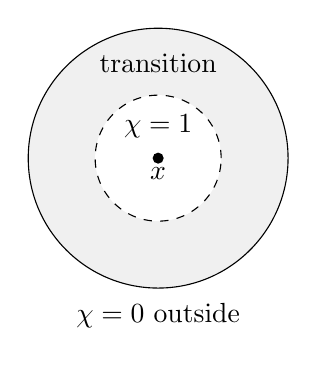
\begin{tikzpicture}[scale=1]
\fill[gray!12] (0,0) circle (1.65);
\fill[white] (0,0) circle (.8);
\draw (0,0) circle (1.65);
\draw[dashed] (0,0) circle (.8);
\fill (0,0) circle (2pt) node[below] {\(x\)};
\node at (0,.4) {\(\chi=1\)};
\node at (0,1.2) {transition};
\node at (0,-2) {\(\chi=0\) outside};
\end{tikzpicture}
\column{.53\textwidth}
Choose a smooth \(\chi\) with \(0\le\chi\le1\).
\par\bigskip
\(\chi=1\) in the small ball.
\par\medskip
\(\chi=0\) outside the larger ball.
\par\medskip
Between them, \(\chi\) changes smoothly from \(1\) to \(0\).
\end{columns}
\end{frame}

\begin{frame}{Step 1: extend the weight by zero}
Define a function on \(X\):
\[
\psi_x=\begin{cases}
a\chi(z)\log|z|&\text{in }U,\\
0&\text{outside }U.
\end{cases}
\]
\textbf{Near \(x\):} \(\psi_x=a\log|z|\).
\par\medskip
\textbf{Near the boundary of \(U\):} \(\psi_x=0\), so extension by zero is smooth there.
\par\medskip
The only singular point is \(x\).
\end{frame}

\begin{frame}{Step 1: modify a metric we already have}
Take a smooth metric \(h_0\) on \(B\). Define
\[
\boxed{h=h_0e^{-2\psi_x}.}
\]
For a local section \(s\), this means
\[
|s|_h^2=|s|_{h_0}^2e^{-2\psi_x}.
\]
We multiply an existing metric by one globally defined scalar function. Thus the formula defines a metric on the whole bundle.
\end{frame}

\begin{frame}{Step 1: check the multiplier ideal}
\textbf{Near \(x\).} Since \(\chi=1\),
\[
e^{-2\psi_x}=e^{-2a\log|z|}=|z|^{-2a}.
\]
The smooth metric \(h_0\) changes the integrand by a locally bounded, positive factor. So the model calculation still applies.
\par\medskip
\textbf{Away from \(x\).} The metric is smooth, so the ideal is \(\cO_X\).
\par\medskip
For \(a=n\), the global multiplier ideal is the ideal sheaf of the point \(x\). For \(a=n+1\), it is its square.
\end{frame}

\begin{frame}{Step 2: what happened to the curvature?}
Recall the local convention
\[
h_0(e,e)=e^{-2\varphi_0},\qquad i\Theta_{h_0}=2i\partial\db\varphi_0.
\]
Our new metric is
\[
h(e,e)=e^{-2\varphi_0}e^{-2\psi_x}=e^{-2(\varphi_0+\psi_x)}.
\]
Differentiate the sum:
\[
\boxed{i\Theta_h=i\Theta_{h_0}+2i\partial\db\psi_x.}
\]
\end{frame}

\begin{frame}{Step 2: near the pole, curvature is nonnegative}
In the small ball, \(\psi_x=a\log|z|\).
\par\bigskip
We know that \(\log|z|\) is psh. Therefore
\[
2i\partial\db\psi_x\ge0
\]
in the sense of currents.
\par\bigskip
Outside the larger ball, \(\psi_x=0\), so this contribution is zero.
\end{frame}

\begin{frame}{Step 2: the cutoff can cost curvature}
On the transition annulus, the function \(\chi\log|z|\) is smooth.
Its curvature contribution need not be positive.
\par\bigskip
But the closed annulus is compact and avoids \(z=0\). Its second derivatives are bounded.
\par\bigskip
Hence there is a finite \(C_1\ge0\) such that, on all of \(X\),
\[
\boxed{2i\partial\db\psi_x\ge-C_1\omega.}
\]
Here \(\omega\) is a fixed smooth Kähler form.
\end{frame}

\begin{frame}{Step 2: now bring in the high power}
Fix a smooth positive metric \(h_L\) on \(L\), and put
\[
\omega=i\Theta_{h_L}>0.
\]
In a local frame write \(h_L=e^{-2\varphi_L}\). On \(L^N\), the induced metric is
\[
h_L^N=(e^{-2\varphi_L})^N=e^{-2N\varphi_L}.
\]
Thus
\[
\boxed{i\Theta_{h_L^N}=2i\partial\db(N\varphi_L)=N\omega.}
\]
Taking the power multiplies the positive curvature by \(N\).
\end{frame}

\begin{frame}{Step 2: the other bundle contributes a fixed error}
Our bundle is \(B=L^N\otimes K_X^{-1}\).
\par\medskip
Choose any smooth metric \(g\) on \(K_X^{-1}\). This metric stays fixed as \(N\) increases.
\par\medskip
On compact \(X\), its curvature has a lower bound
\[
i\Theta_g\ge-C_0\omega
\]
for some finite \(C_0\ge0\).
\par\medskip
The product metric \(h_0=h_L^N g\) on \(B\) therefore satisfies
\[
i\Theta_{h_0}=N\omega+i\Theta_g\ge(N-C_0)\omega.
\]
\end{frame}

\begin{frame}{Step 2: put the three contributions together}
The singular metric on \(B=L^N\otimes K_X^{-1}\) is
\[
h=h_L^N g\,e^{-2\psi_x}.
\]
Its curvature satisfies
\[
\begin{aligned}
i\Theta_h
&=\underbrace{N\omega}_{\text{positive power}}
 +\underbrace{i\Theta_g}_{\ge-C_0\omega}
 +\underbrace{2i\partial\db\psi_x}_{\ge-C_1\omega}\\[8pt]
&\ge(N-C_0-C_1)\omega.
\end{aligned}
\]
Choose \(N>C_0+C_1\). Then Nadel's positivity hypothesis holds.
\end{frame}

\begin{frame}{Step 3: one exponent must work everywhere}
So far we fixed one point \(x\). An embedding needs one bundle \(L^N\) that works for \textbf{every} point.
\par\bigskip
Use finitely many coordinate charts covering compact \(X\). Inside each chart, use cutoffs of one fixed radius, translated to the different centres.
\par\bigskip
Their transition annuli stay a fixed distance from the pole. Their derivative bounds are uniform.
\par\medskip
Taking the largest of finitely many bounds gives one \(C_1\), valid for every centre and both coefficients \(n,n+1\).
\src{The coordinate-cover details are in the appendix.}
\end{frame}

\begin{frame}{Step 3: to separate two points, use two poles}
Fix \(x\ne y\). At each point use coefficient \(a=n\), and add the two weights:
\[
\psi=\psi_x+\psi_y,\qquad
h=h_L^Ng\,e^{-2(\psi_x+\psi_y)}.
\]
Near \(x\), the function \(\psi_y\) is smooth. It does not change integrability there, so the ideal is \(\mathfrak m_x\).
\par\medskip
Near \(y\), the ideal is \(\mathfrak m_y\). Elsewhere the metric is smooth.
\[
\boxed{\cI(h)=\mathfrak m_x\cap\mathfrak m_y.}
\]
\end{frame}

\begin{frame}{Step 3: the curvature costs add}
Each pole contributes at worst \(-C_1\omega\). For two poles,
\[
2i\partial\db(\psi_x+\psi_y)\ge-2C_1\omega.
\]
Thus
\[
i\Theta_h\ge(N-C_0-2C_1)\omega.
\]
\textbf{Choose one integer \(N>C_0+2C_1\).}
\par\medskip
It works for one value, two values, and first derivatives, at every point.
The supports of the two cutoffs may overlap.
\end{frame}

\begin{frame}{Step 3: now apply Nadel}
For that one \(N\), we have constructed metrics on \(B=L^N\otimes K_X^{-1}\) with
\[
\cI(h)=\mathfrak m_x,\quad\mathfrak m_x\cap\mathfrak m_y,
\quad\text{or}\quad\mathfrak m_x^2.
\]
Each has strictly positive curvature. Nadel gives
\[
H^1(X,K_X\otimes B\otimes\cI(h))=0.
\]
Cancel \(K_X\otimes K_X^{-1}\):
\[
\boxed{H^1(X,L^N\otimes I)=0\text{ for each required ideal }I.}
\]
\end{frame}

\begin{frame}{Step 4: from vanishing to prescribed data}
Put \(A=L^N\). Tensor the ideal sequence by \(A\):
\[
0\longrightarrow A\otimes I\longrightarrow A
\longrightarrow A\otimes(\cO_X/I)\longrightarrow0.
\]
The long exact sequence contains
\[
H^0(X,A)\longrightarrow H^0(X,A\otimes\cO_X/I)
\longrightarrow\underbrace{H^1(X,A\otimes I)}_{0}.
\]
Exactness says the first arrow is surjective.
\par\medskip
So any datum in the quotient comes from a global section.
\end{frame}

\begin{frame}{Step 4: no base points}
Take \(I=\mathfrak m_x\). The quotient remembers only the value at \(x\):
\[
H^0(X,A\otimes\cO_X/\mathfrak m_x)=A|_x.
\]
Surjectivity says that any element of this one-dimensional fibre is the value of a global section.
\par\medskip
Choose a nonzero value. Some global section is nonzero at \(x\).
\par\medskip
Since this works for every \(x\), the sections have no common zero. The projective map is defined everywhere.
\end{frame}

\begin{frame}{Step 4: what does separates points mean?}
\textbf{Definition.} Sections of \(A\) separate points if, for every \(x\ne y\), some global section satisfies
\[
s(x)=0,\qquad s(y)\ne0.
\]
To find such a section, use \(I=\mathfrak m_x\cap\mathfrak m_y\). The evaluation map is
\[
H^0(X,A)\longrightarrow A|_x\oplus A|_y,\qquad
s\longmapsto(s(x),s(y)).
\]
This target is a vector space of dimension two, one fibre at each point.
\par\medskip
Surjectivity lets us prescribe \((0,b)\), with \(b\ne0\).
\end{frame}

\begin{frame}{Step 4: why point separation gives injectivity}
Choose a basis \(t_0,\ldots,t_M\) of \(H^0(X,A)\). In fibre coordinates,
\[
\Phi(x)=[t_0(x):\cdots:t_M(x)].
\]
Suppose \(\Phi(x)=\Phi(y)\). Then, for some nonzero scalar \(\lambda\),
\[
t_j(y)=\lambda t_j(x)\qquad\text{for every }j.
\]
Every section is a linear combination of this basis. So \(s(y)=\lambda s(x)\) for every \(s\).
\par\medskip
This contradicts the section with \(s(x)=0\), \(s(y)\ne0\). Hence \(\Phi\) is injective.
\end{frame}



\begin{frame}{Step 4: lift the simplest first jets}
Use \(I=\mathfrak m_x^2\). In a local frame of \(A\), prescribe the first jets
\[
1,\quad z_1,\quad\ldots,\quad z_n.
\]
Lift them to global sections \(s_0,s_1,\ldots,s_n\). Locally they satisfy
\[
s_0=1+O(|z|^2),\qquad s_j=z_j+O(|z|^2).
\]
The error terms have zero value and zero first derivatives at \(x\).
\par\medskip
These sections are linearly independent, so extend them to a basis of \(H^0(X,A)\).
\end{frame}

\begin{frame}{Step 4: the differential is injective}
Since \(s_0(x)=1\), we can use the affine projective chart where \(s_0\ne0\).
Coordinates of our map include
\[
\frac{s_j}{s_0}=z_j+O(|z|^2).
\]
Taking the differential at \(x\) gives
\[
d\!\left(\frac{s_j}{s_0}\right)_x=dz_j.
\]
If \(d\Phi_x(v)=0\), all \(dz_j(v)\) vanish, so \(v=0\).
\par\medskip
Thus the map is an immersion. This is \textbf{separation of tangent directions}.
\end{frame}

\begin{frame}{Kodaira embedding: conclusion}
We have constructed an everywhere-defined injective holomorphic immersion
\[
\Phi_N:X\longrightarrow\Pj(H^0(X,L^N)^*).
\]
Since \(X\) is compact and projective space is Hausdorff, \(\Phi_N\) is a homeomorphism onto its image. Together with immersion, this gives
\[
\boxed{\Phi_N\text{ is a holomorphic embedding}.}
\]
Conversely, the restricted Fubini--Study metric is positive.
\par\medskip
We have proved the destination announced in lecture 23 (Daniel).
\end{frame}

\begin{frame}{Chow's theorem: the image is algebraic}
\textbf{Chow.} Every closed complex analytic subvariety \(Y\subset\Pj^M\) is algebraic.
\par\bigskip
Thus our compact embedded image is the common zero set of finitely many homogeneous polynomials:
\[
\boxed{\Phi(X)=\{F_1=\cdots=F_r=0\}\subset\Pj^M.}
\]
A single equation is the hypersurface case. In higher codimension we generally need several equations.
\src{HP, complex-geometry.tex, section-chow-theorem. Mauri, \emph{Kodaira Embedding Theorem}, Section 12.}
\end{frame}

\begin{frame}{Chow's theorem in a picture}
\begin{center}
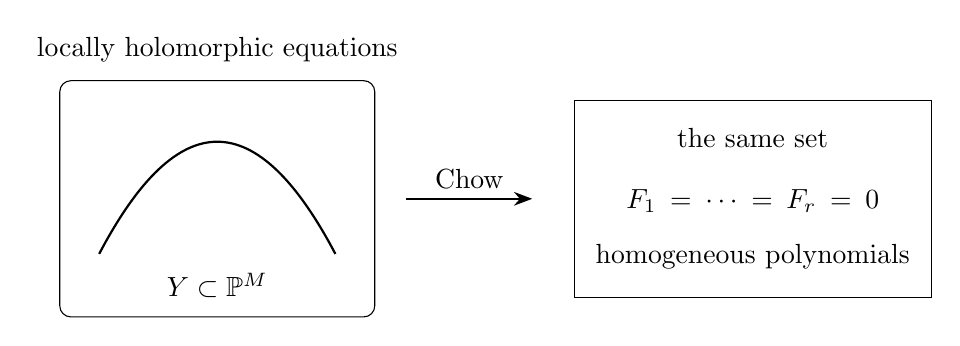
\begin{tikzpicture}[>=Stealth]
\draw[rounded corners] (-5,-1.5) rectangle (-1,1.5);
\draw[thick] (-4.5,-.7) .. controls (-3.5,1.2) and (-2.5,1.2) .. (-1.5,-.7);
\node at (-3,-1.1) {\(Y\subset\Pj^M\)};
\node at (-3,1.9) {locally holomorphic equations};
\draw[->,thick] (-.6,0)--(1,0) node[midway,above] {Chow};
\node[draw,align=center,text width=4.3cm,minimum height=2.5cm] at (3.8,0)
{the same set\\[10pt]\(F_1=\cdots=F_r=0\)\\[8pt]homogeneous polynomials};
\end{tikzpicture}
\end{center}
\par\bigskip
Analysis constructed the embedding. Chow identifies its image as a projective algebraic variety.
\src{Original mathematical illustration, not a portrait.}
\end{frame}

\begin{frame}{Chow, step 1: hypersurfaces give line bundles}
A complex hypersurface \(Y\) is locally cut out by one holomorphic equation \(f_i=0\).
On overlaps, these equations differ by nowhere-zero holomorphic factors.
\par\medskip
Those factors define a line bundle \(\cO(Y)\) and a global holomorphic section \(s_Y\) whose zero set is \(Y\).
\par\medskip
On projective space,
\[
\operatorname{Pic}(\Pj^M)=\mathbb Z[\cO(1)].
\]
Thus \(\cO(Y)\simeq\cO(d)\) for an integer \(d\).
\src{HP: exercise-pic-of-pn-is-z and section-chow-theorem.}
\end{frame}

\begin{frame}{Chow, step 2: why the Picard group is the integers}
The exponential sequence gives
\[
H^1(\Pj^M,\cO)\longrightarrow\operatorname{Pic}(\Pj^M)
\xrightarrow{c_1}H^2(\Pj^M,\mathbb Z)\longrightarrow H^2(\Pj^M,\cO).
\]
The outer groups vanish, while \(H^2(\Pj^M,\mathbb Z)\simeq\mathbb Z\).
Therefore \(c_1\) is an isomorphism.
\par\medskip
The class of \(\cO(1)\) is the generator, so every holomorphic line bundle is some \(\cO(d)\).
\par\medskip
We use the usual cohomology of projective space and its Hodge decomposition here.
\end{frame}

\begin{frame}{Chow, step 3: holomorphic sections become polynomials}
A section of \(\cO(d)\) lifts to a holomorphic function \(F\) on \(\C^{M+1}\setminus\{0\}\), with
\[
F(\lambda Z)=\lambda^dF(Z).
\]
Hartogs extends \(F\) across \(0\), for \(M\ge1\).
\par\medskip
Expand at \(0\): \(F=\sum_{k\ge0}P_k\), with \(P_k\) homogeneous of degree \(k\).
The scaling identity forces \(P_k=0\) for \(k\ne d\).
\[
\boxed{F=P_d\text{ is a homogeneous polynomial}.}
\]
This is where Hartogs enters the HP proof.
\src{HP: theorem-secti-od-degre-d-homog-poly.}
\end{frame}

\begin{frame}{Chow, step 4: higher codimension needs projection}
Work with an irreducible \(Y\), of dimension \(k<M-1\), and take \(p\notin Y\).
\par\medskip
\textbf{Projection lemma (input).} Choose a linear projection to \(\Pj^{k+1}\), defined on \(Y\) and \(p\), whose image of \(Y\) is an analytic hypersurface avoiding the image of \(p\).
\par\medskip
The hypersurface case gives a homogeneous equation downstairs. Pulling it back gives a homogeneous polynomial that vanishes on \(Y\) but not at \(p\).
\par\medskip
This is a proof sketch: generic projection and analyticity of the proper image are additional analytic-geometric inputs.
\src{HP, section-chow-theorem; Mauri, Section 12. Proper-image analyticity uses Remmert's theorem.}
\end{frame}

\begin{frame}{Chow, conclusion: finitely many equations}
For each \(p\notin Y\), we obtained a homogeneous polynomial \(F_p\) with
\[
F_p|_Y=0,\qquad F_p(p)\ne0.
\]
Thus the common zero set of all these polynomials is exactly \(Y\).
\par\medskip
The homogeneous ideal they generate in \(\C[Z_0,\ldots,Z_M]\) is finitely generated, by the Hilbert basis theorem.
\[
\boxed{Y=V(F_1,\ldots,F_r).}
\]
We have reached actual homogeneous polynomial equations.
\end{frame}

\begin{frame}{From an estimate to an algebraic variety}
\begin{enumerate}
\setlength{\itemsep}{12pt}
\item Positive curvature gives a weighted \(L^2\) estimate.
\item The Hilbert-space argument turns it into a solution of \(\db u=f\).
\item Subtracting \(u\) produces holomorphic sections with prescribed data.
\item Those sections give an injective immersion. Compactness gives an embedding.
\item Chow turns the closed analytic image into a projective algebraic variety.
\end{enumerate}
\par\medskip
This completes the main argument of our two lectures.
\end{frame}

\end{document}
